\batchmode
\documentclass{article}
\usepackage{tikz}

\providecommand{\checkpointformat}{}
\checkpointformat

\begin{document}

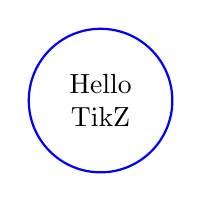
\begin{tikzpicture}
    \node[draw=blue, thick, circle, inner sep=8pt, align=center ] at (0,0) {Hello\\TikZ};
\end{tikzpicture}

\newcommand{\plotRange}{5.5}
\newcommand{\plotSamples}{35}
\newcommand{\gridDensity}{25}

\begin{tikzpicture}[x={(0.866cm,-0.25cm)}, y={(0.5cm,0.4cm)}, z={(0cm,1.0cm)}]
  \foreach \i in {-\gridDensity,...,\gridDensity} {
    \pgfmathsetmacro{\u}{\plotRange * \i / \gridDensity}
    \draw[blue!70!black, thin] plot[domain=-\plotRange:\plotRange, samples=\plotSamples] 
      (\u, \x, {3 * (1 - 0.25*(\u*\u + \x*\x)) * exp(-0.125*(\u*\u + \x*\x))});
    \draw[red!70!black, thin] plot[domain=-\plotRange:\plotRange, samples=\plotSamples] 
      (\x, \u, {3 * (1 - 0.25*(\x*\x + \u*\u)) * exp(-0.125*(\x*\x + \u*\u))});
  }
\end{tikzpicture}

\end{document}
